\chapter{Pairwise Graph Convolutional Networks for Interface Prediction}
\label{chap:methods}

The methods presented in this thesis were motivated by a desire to exploit the local structure around a residue when performing interface prediction.
The biological reasoning for this is that a residue's neighborhood influences its propensity to participate in an interface.
It was noted in Chapter \ref{chap:neuralnetworks} that convolutional neural networks are one way of detecting features in a local neighborhood, but they are limited to regular grids. 
Unfortunately, proteins cannot naturally be represented as a regular grid, so convolution must be developed for a more natural representation: graphs.


\section{Proteins As Graphs}

An undirected, unweighted graph $G$ consists of a set of vertices, $V=\{v_1, v_2, ..., v_n\}$, and a set of eges, $E=\{e_1, e_2, ..., e_m\}$ where each edge is incident to two vertices and there is at most one edge between two vertices.
One way of representing proteins as graphs is to let each vertex represent a residue in the protein, and each edge represent the relationship between two residues.
Thus any information pertaining to a particular residue can be associated with the relevant vertex in the form of a feature vector.
The features used in this work are drawn from features used in prior interface prediction work \cite{minhas2014}.
Likewise, any information about the relationship between two residues can be associated with the relevant edge.
The edge features used here describe the distance between and relative orientation of two residues.
These edge features are defined between any two residues in the protein, so the graph is complete. 
A detailed explanation of each feature is contained in Appendix \ref{appendix:features}

This representation is an abstraction of the original protein to a well studied mathematical object, with two notable facts.
First, the graph itself does not rely on a coordinate system, as is the case when working with raw 3D positions.
Second, the features contained on the graph are also not tied to a coordinate system, since they simply describe attributes of residues or pairs of residues.
These facts make a protein graph invariant to rotations or translations in space. 
However, since the graph was constructed from points in 3D space, local neighborhoods of vertices can be defined using spatial proximity.
This is useful when designing convolutions that use a local neighborhood as a receptive field.
With proteins represented as graphs, the remaining task is to design a convolution which operates on graphs. 

\section{Graph Convolution}
Recent years have seen increased attention to problems involving graph structured data, prompting developments in graph convolution to perform various tasks on those data~\cite{bronstein2016}.
These developments allow leveraging of deep learning techniques, which have shown great success for problems on regular grids.
Though each variant of graph convolution is tailored to suit the data and problem being addressed, there are some common approaches which merit describing generally.
These approaches generally fall into one of two categories: \emph{spectral} or \emph{spatial}


\subsection{General Approaches}
Spectral methods of graph convolution are based on linear functions in the "frequency domain" of a graph, defined using the laplacian operator $\mathcal{L}=I-D^{-1/2}WD^{-1/2}$, where $I$ is the identity matrix, $W$ is a similarity matrix (containing scalar edge weights), and $D$ is a diagonal matrix containing the degree of each vertex~\cite{bruna2013, henaff2015, kipf2016}.
Each filter in a spectral convolution implies a weighting of each frequency in the spectral decomposition of the graph~\cite{mallat2009}.
In physics, the Laplacian operator is used to model the diffusion of a gas in a volume.
In a similar way, the graph Laplacian can be thought of as modeling diffusion along the edges of the graph.

Spatial approaches instead define operations in a localized neighborhood of a central vertex~\cite{henaff2015, atwood2016}.
Each neighborhood constitutes a receptive field where a convolution operation is performed (see Figure \ref{fig:spatial_graph_conv}).
Spatial convolution commonly involves a vector of weights and takes a weighted sum of neighbors, much like a discrete convolution on a grid can be viewed as taking a weighted sum of grid elements within the receptive field.
Spatial convolution is more directly analogous to grid based convolution as described in Chapter \ref{chap:neuralnetworks}.
Unlike grids, however, spatial graphs suffer from a problem of receptive field correspondence.

\begin{figure}
	\centering
	%\begin{center}
	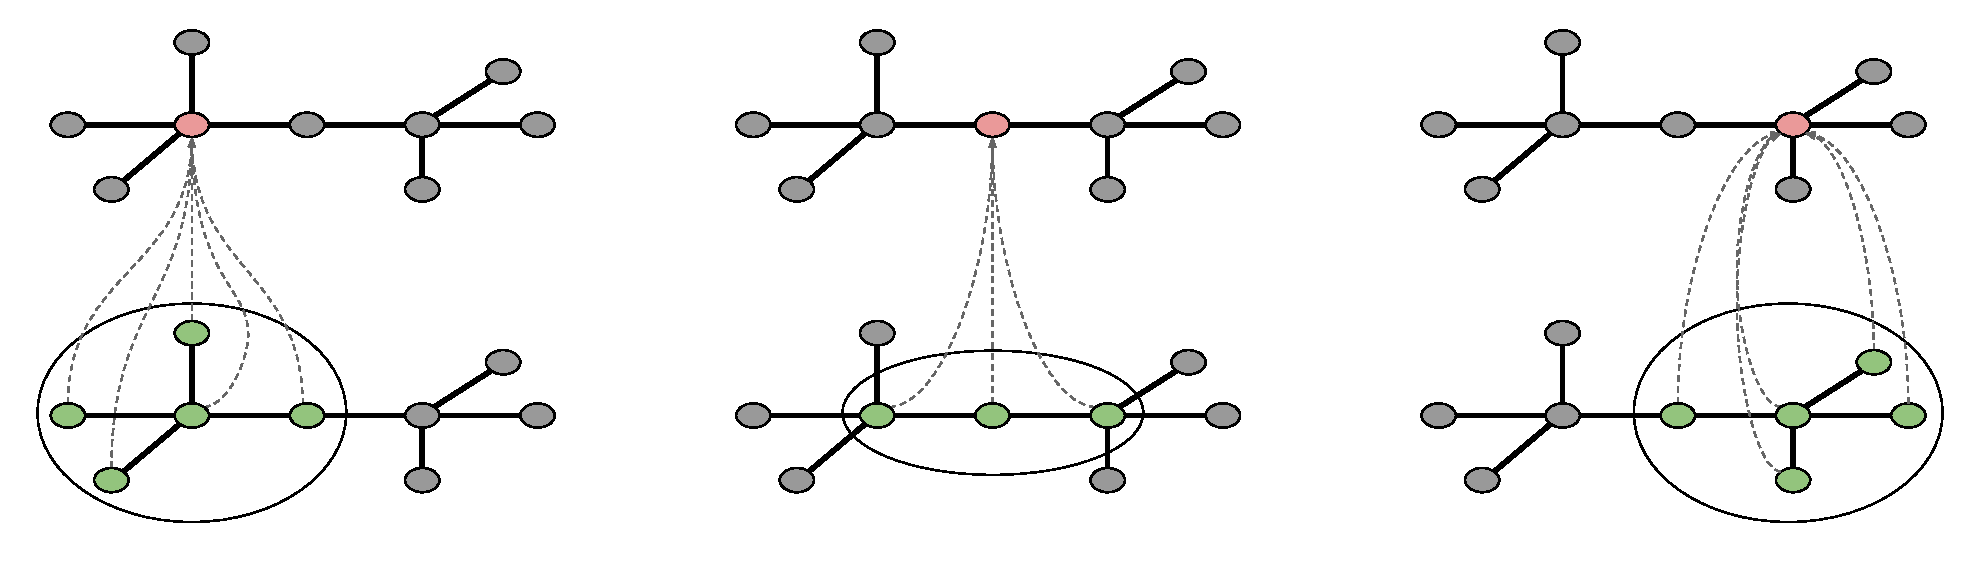
\includegraphics[width=\textwidth]{conv_graph.pdf}
	%\end{center}
	\caption{An example of spatial graph convolution, defining receptive fields around a central vertex. The result of convolution is applied to the central vertex in the receptive field.}
	\label{fig:spatial_graph_conv}
\end{figure}

\subsection{Receptive Field Correspondence in Spatial Convolution}


When convolving on a grid, each receptive field has an identical structure, so each pixel in a receptive field can be associated with a unique pixel in a different one.
Therefore the same set of weights can be applied to each receptive field such that each weight is always applied to the same region within the receptive field.
With graphs, there is often no such correspondence from one receptive field to another, since vertices are inherently unordered.
The central vertices may be associated, but the number of neighbors may not even be the same, depending on how the receptive field is defined. 
Hence the consistent application of weights across receptive fields is only possible after these issues have been addressed.
This is typically done in one of two ways:

\begin{enumerate}
	\item \textit{Imposed ordering of neighbors}. This approach establishes a correspondence between two receptive fields by ordering the neighbors in each and associating neighbors of a common position. 
	Ordering methods are either based on vertex characteristics, like degree and betweenness centrality, or domain specific knowledge ~\cite{niepert2016, duvenaud2015}.
	They typically require the number of neighbors in a receptive field to remain the same.
	This approach allows filter weights which are applied to a particular position in the ordering, which, it is assumed, has some significance across all receptive fields.
	If the imposed ordering is arbitrary, this approach has limited usefulness.
	Methods following this approach can be called \emph{ordered}.
	
	\item \textit{Identical treatment of neighbors}. This approach ignores the need to establish a correspondence between receptive fields and instead treats all neighbors identically.
	Rather than apply different weights to neighbors depending on their position in an ordering, the same weights are applied to each neighbor.
	This allows for different sizes of receptive fields and avoids choosing an ordering method, but lacks the ability to treat each neighbor uniquely.
	Methods following this approach can be called \emph{order free}.
\end{enumerate}

Figure \ref{fig:correspondence_approaches} depicts both approaches.
Examples of each were evaluated for this thesis.
In addition, novel convolutions were examined which attempt to incorporated the advantages of both ordered and order free methods.
Below is a description of each existing method followed by the novel methods presented in this thesis. 

\begin{figure}
	\centering
	%\begin{center}
	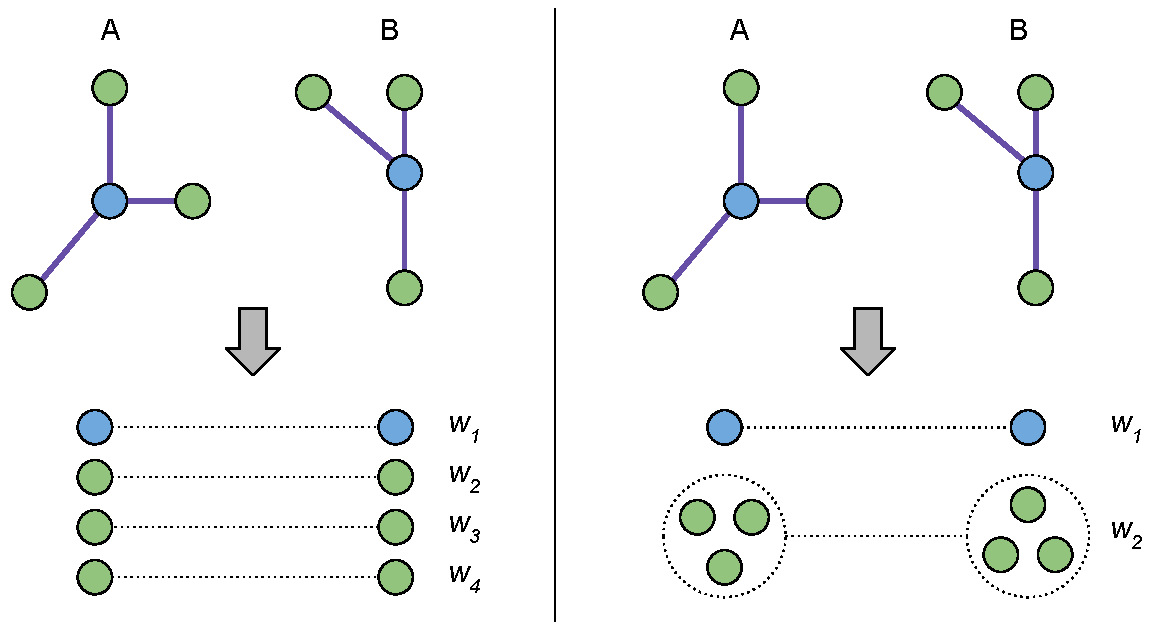
\includegraphics[width=0.8\textwidth]{correspondence_approaches.pdf}
	%\end{center}
	\caption{Two approaches of establishing correspondence between the neighbors of receptive fields A and B. Central vertices are shown in blue and neighbors in green. The central vertices always correspond with one another. Left: neighbors are ordered and associated based on position. Unique weights (\textit{$w_2$--$w_4$}) can then be applied to each position in the order. Right: neighbors are left unordered and treated identically. This requires that the same weights (\textit{$w_2$}) be used for all neighbors.}
	\label{fig:correspondence_approaches}
\end{figure}


\subsection{Diffusion Based Method}
As mentioned, spectral methods utilize the Laplacian operator, which is used to model diffusion processes. 
Although no spectral methods were examined in this thesis, a non-spectral diffusion method was.
Atwood and Towsley (2016)~\cite{atwood2016} propose a Diffusion Convolutional Neural Network (DCNN) which uses a graph's similarity matrix into a transition matrix by normalizing rows.
The transition matrix $P$ is raised to successive exponents, generating a power series, with each power corresponding to random walks of length equivalent to that power.
For a maximum power of $L$, the activation of a node is:

\begin{equation}
h(x_i | W^\textsc{c}) = \sigma \bigg( \sum_{l=0}^L (W^\textsc{c}_{l\cdot} \odot P^l X ) \bigg),
\label{eq:diffusion}
\end{equation}

\noindent
where $W^\textsc{c}$ is a matrix of weights, $\odot$ denotes broadcasted elementwise multiplication, and $X$ is a matrix of all vertices, where each row is a vertex and each column a different feature.
For each power $l$, all vertices that have a random walk of length $l$ that end at the vertex of interest are summed together, weighted by the walk probability.
This sum is then multiplied elementwise with a weight vector and summed with the result of all other powers to produce the overall signal.
Unlike other convolutions presented here, this method does not use a receptive field, instead relying on the similarity matrix to indicate proximity.


\subsection{Ordered Method}

Niepert et al (2016)~\cite{niepert2016} describe an ordered graph convolution that is used in their tool, \emph{PATCHY-SAN}, which performs classification at the graph level.
This method first performs a graph labeling procedure to globally order the vertices.
This ordering is traversed with a given stride to select a subset of vertices which serve as the centers of convolutions.
Local neighborhoods are constructed for each central vertex and ordered according to a \emph{normalization} procedure.
The ordered vertices serve as the receptive field for convolution at the central vertex, which is also in the ordering. 
If $(x_1, x_2, ... , x_k)$ is the ordered list of vertices, then convolution takes the form:

\begin{equation}
h(x_i | \{ W_{j} \}, b)= \sigma \bigg( \frac{1}{k} \sum_{j=1}^{k}(W_{j} x_j) + b \bigg),
\label{eq:patchysan}
\end{equation}

\noindent
where $\{W_j\}$ is the set of weight matrices to use on each member of the receptive field.
A natural ordering technique is one which places the center vertex first and orders its neighbors from least to greatest distance from the center. 
In this way, one weight matrix is used for all center vertices, another for all nearest neighbors, etc.
The vertex ordering also imposes a lexicographic ordering on the neighborhood edges as well, so unique weights can be used to generate a signal from each edge. 
Adding this term to the convolution generates:

\begin{equation}
h(x_i | \{ W_{j} \}, \{ W_{jk} \}, b)= \sigma \bigg( \frac{1}{k} \sum_{j=1}^{k}(W_{j} x_j) + \frac{1}{k^2} \sum_{j = 1}^{k-1} \sum_{l=j+1}^{k}(W_{jk} A_{jk})  + b \bigg),
\label{eq:patchysan_2e}
\end{equation}

\noindent
where $W_{jl}$ is the weight matrix associated with edge $(j, l)$ in the lexicographic ordering.
Originally, Niepert et al use the graph ordering to construct a one dimensional grid from the output of graph convolution, separately for vertices and edges.
They then perform traditional convolution on the results until classifying the graph as a whole.
For interface prediction however, the edges and vertex signals are averaged together and applied to the central vertex so that repeated graph convolutions may be performed without losing the graph structure, and no graph labeling is necessary.


\subsection{Order Free Methods}
One of the simplest forms of order free graph convolution was proposed by Duvenaud and Maclaurin, et al (2015)~\cite{duvenaud2015}, which was used for generating molecular \emph{fingerprints}.
This method uses a single set of weights for all vertices in the receptive field, including the central vertex:

\begin{equation}
h(x_i | W, b)= \sigma \bigg( W \sum_{j \in \mathcal{F}}x_j + b\bigg),
\label{eq:fingerprint}
\end{equation}

\noindent
where $\mathcal{F}$ is the index set of all vertices in the receptive field.
In the original formulation, no bias term was included
However, when used for interface prediction, the version with bias consistently performed better.

As mentioned, center vertices may be treated separately from the neighbors, even if all neighbors are treated identically. 
Schlichtkrull and Kipf (2017)~~\cite{schlichtkrull2017}) proposed such an approach called \emph{Relational Graph Convolutional Networks}, or R-GCN.
Their methods were developed for use in knowledge bases, graph structures where the vertices are named entities and the edges capture the many binary relationships between the entities. 
To convolve a vertex, they take the neighborhood defined by each relation type and sum the signal from all the neighbors in that neighborhood.
The resultant signal is the sum of signals from all neighborhoods.
For protein graphs, spacial proximity is the only method for determining neighborhoods that makes sense biologically, so there is only one neighborhood.
The adapted version of this convolution for use in interface prediction is:

\begin{equation}
h(x_i | W^\textsc{c}, W^\textsc{n}, b)= \sigma \bigg( W^\textsc{c} x_i + \frac{1}{|\mathcal{N}_i|} \sum_{j \in \mathcal{N}_i}(W^\textsc{n} x_j)  + b\bigg),
\label{eq:rgcn}
\end{equation}

\noindent
where separate weights are used for the center and neighbors. 
In the original version, a different weight matrix was used for each of the many relation types.  
To reduce the number of model parameters, all weight matrices were simply linear combinations of a set of learnable basis weight matrices:

\begin{equation}
W^\textsc{(c, n)} = \sum_{b} a^\textsc{(c, n)}_b V_b 
\label{eq:rgcn_basis}
\end{equation}

\noindent
where $\{V_b\}$ is a set of basis functions, $a^\textsc{c}$ and $a^\textsc{n}$ are scalar weights that combine the basis functions to create $W^\textsc{c}$ and $W^\textsc{n}$, respectively.
R-GCNs were examined with and without basis functions.

The above order-free methods do not incorporate edge information.
Sch{\"u}tt et al (2016)~\cite{schutt2017} propose a version called \emph{Deep Tensor Networks} (DTN) which creates a signal for the neighbor vertices as well as the edges which connect them to the central vertex:

\begin{equation}
h(x_i | W, W^\textsc{n}, W^\textsc{e}, b^\textsc{n}, b^\textsc{e})= x_i + \sum_{j \in \mathcal{N}_i} \sigma \bigg[ W \bigg( (W^\textsc{n} x_j + b^\textsc{n}) \odot (W^\textsc{e} A_{ij} + b^\textsc{e}) \bigg) \bigg],
\label{eq:deep_tensor}
\end{equation}

\noindent
where $A_{ij}$ are the features for edge $(i, j)$, and $\odot$ denotes the elementwise product.
In this formulation, $W^\textsc{n}$ and $W^\textsc{e}$ transform vertices and edges respectively into a common dimensional space, and $W$ transforms their combination back into the dimensionality of the input. 
This convolution does not transform the input by any weight matrix, rather it can be viewed as updating the representation at $x_i$ using information from its neighbors.
This restricts representations to always have the same dimensionality, which is not true in grid convolutions. 
Ideally, the central vertex would have a weight matrix.
Nevertheless, this method uniquely incorporates edge information, so that even while all neighbors use the same weight matrix, the information on their edges is used to differentiate them.
This concept is carried forward into the novel convolution methods presented below.


\subsection{Novel Order-Free Methods}
Like DTN, these methods incorporate edge information to help differentiate neighbors, but also avoid imposing an arbitrary ordering on the neighbors in a receptive field.
This is accomplished by incorporating information from the edges between each neighbor and the central vertex.
Here are two variants of graph convolution which differ only in how the edge information is incorporated, denoted \textit{Sum Coupling} and \textit{Product Coupling}.
For a central vertex $i$ on the graph and a local neighborhood of vertices $\mathcal{N}_i$, the output of \emph{Sum Coupling} graph convolution is:
\begin{equation}
h(x_i | W^\textsc{c}, W^\textsc{n}, W^\textsc{e}, b) = \sigma \bigg( W^{\textsc{c}} x_i + \frac{1}{|\mathcal{N}_i|}\sum_{j \in \mathcal{N}_i} (W^{\textsc{n}} x_j + W^{\textsc{e}} A_{ij}) + b \bigg),
\label{eq:sum_coupling}
\end{equation}
where $x_i$ is the feature vector associated with vertex $i$, $A_{ij}$ is the feature vector associated with edge $(i, j)$, $W^\textsc{c}$, $W^\textsc{n}$ and $W^\textsc{e}$ are weight matrices, and $b$ is a vector of biases. 
If there are $l$ vertex channels, $p$ edge channels, and $k$ filters, then $W^\textsc{c}\in\mathbb{R}^{k \times l}$, $W^\textsc{n}\in\mathbb{R}^{k \times l}$, $W^\textsc{e}\in\mathbb{R}^{k \times p}$, and $b\in\mathbb{R}^{k}$.
Intuitively, this calculates an activation for the central vertex, each neighbor vertex, and each edge between a neighbor and the central vertex separately.
It is the inclusion of edge activations that allows each neighbor to be distinguished from the others on the basis of its relationship to the central vertex.
This variant is called Sum Coupling because the neighbor vertex and edge activations are added together.
Because of this, the direct association between a neighbor its edge is lost.
A variant which maintains the association is \emph{Product Coupling}, whose output is:
\begin{equation}
h(x_i | W^\textsc{c}, W^\textsc{n}, W^\textsc{e}, b) = \sigma \bigg( W^{\textsc{c}} x_i + \frac{1}{|\mathcal{N}_i|}\sum_{j \in \mathcal{N}_i} (W^{\textsc{n}} x_j \odot W^{\textsc{e}} A_{ij}) + b \bigg),
\label{eq:prod_coupling}
\end{equation}
where $\odot$ denotes the elementwise product between two vectors or matrices. 
This allows a neighbor's influence on the overall activation to be modulated by its relationship to the central vertex.
For protein graphs, this means neighboring residues will contribute more or less to the overall activation, depending on their distance from and relative orientation to the central vertex, with the precise modulation determined by the edge activations.
Note the similarity to Equation (\ref{eq:deep_tensor}).

Just as convolution on a regular grid can be applied at any pixel in an image, graph convolution can be applied to any vertex in the graph.
Hence both can be considered translation invariant.

Both Sum Coupling and Product Coupling graph convolution are translation invariant, don't impose an ordering in the neighbors or a correspondence between receptive fields of any kind, allow for different numbers of neighbors, and account for the different relationships between neighbors and the central vertex. 
The receptive fields are always defined around a central vertex, so the results of convolution can be applied to that vertex.
This retains the graph structure after each convolution, so convolutional layers are stackable, as with images.

A note on receptive fields: protein graphs are complete and embedded in a metric space, so this thesis defines a receptive field using a fixed number of closest neighbors to the central vertex.
A receptive field can also be defined using a threshold $\delta>0$ such that all vertices closer to the central vertex than the threshold are included in the receptive field.
All neighbors in a receptive field are guaranteed to share an edge with the central vertex, allowing the application of equations (\ref{eq:sum_coupling}) and (\ref{eq:prod_coupling}).
For incomplete graphs, a receptive field can be defined as all vertices within $k$ hops of the central vertex. 
If $k=1$, both versions of graph convolution can directly be applied.
If $k>1$, then Product Coupling graph convolution can't be directly applied to neighbors more than 1 hop away from the center vertex, since they share no edge with the center. 
Though there are ways to adapt Product Coupling graph convolution in this situation, they are not the focus of this thesis.
%TODO: say more?

Lastly, to assess the benefit that incorporating information from neighboring residues has on classification performance, the \emph{no convolution} variant is defined as:

\begin{equation}
h(x_i | W^\textsc{c}, b)= \sigma \bigg( W^{\textsc{c}} x_i + b \bigg),
\label{eq:no_conv}
\end{equation}

\noindent
which resembles the activation of a dense layer in regular neural networks.


\section{Pairwise Neural Network Architecture}
These graph convolution operations allow the detection of local patterns on a single graph, and produce a new representation at each vertex.
Partner specific protein interaction, however, requires classifying pairs of residues in different proteins (vertices in different graphs), which is essentially making predictions on vertices in the product graph. 
Such predictions are made using a pairwise neural network architecture.

A pairwise architecture consists first of two identical convolutional modules, each responsible for generating the representation for one of the proteins in the pair.
A key requirement for the pairwise architecture is symmetry, since the prediction for a pair of residues should be the same irrespective of which leg is used for each protein.
To ensure symmetry in the convolution layers, weights are shared between layers in the different legs.
The merge layer then combines the vertex representations from one graph with the vertex representations from the other into pairs.
To maintain symmetry, this merge process should also be symmetric.
For example, the elementwise sum, elementwise product, and outer-product are all commutative and therefore produce symmetric output.
Another option is to combine pairs asymmetrically, such as concatenating the two representations together, but then average the predictions from each ordering of the representations.
%TODO: talk about pairwise kernels?
Finally, the combined representation for each pair of residues is passed through a number of fully connected layers.
The data are represented as pairs of residues at this point. 
Theoretically, graph convolution could be performed at this stage as well, this time in the product graph.
However, the computational and memory requirements of doing so prove prohibitive since the number of convolutions and the number of neighbors in each convolution increases quadratically.
Hence the work in this thesis performs no convolution after merging.
The final layer has a single output for each pair indicating the prediction for that pair.
See Figure \ref{fig:pairwise_arch1} for a graphical depiction.

This output is converted to a binary class prediction vector using a softmax function, 

\begin{equation}
\text{softmax}(x) = \bigg[ \frac{e^{-x}}{e^{x} + e^{-x}} , \frac{e^{x}}{e^{x} + e^{-x}} \bigg],
\label{eq:softmax}
\end{equation}

\noindent
the elements of which can be interpreted as class probabilities for the negative (non-interfacial) and positive (interfacial) classes, respectively.
This output is compared to a one-hot label vector indicating whether \big($[0, 1]$\big) or not\big($[1, 0]$\big) the pair constitute part of the true interface. 

\begin{figure}
	\includegraphics[width=\textwidth]{pairwise_network4.pdf}
	\caption{A pairwise neural network architecture that takes two protein graphs as input. Each leg contains one or more convolutional layers. The resultant graphs are then merged to create representations of residue pairs. After more fully connected layers, a final classification is performed for each pair.}
	\label{fig:pairwise_arch1}
\end{figure}


This chapter has presented protein graphs, graph convolution operations, and pairwise neural network architectures, all of which are components in this deep learning approach partner specific protein interface prediction.
Chapter \ref{chap:experiments} describes the experiments that were performed and gives a discussion of the results.
